\title{Getting Started}

\subsection{Getting Started}
Getting started with Edward is easy.

\subsubsection{Quick Installation}
\textbf{Warning: TensorFlow v0.12.0rc0 and v0.12.0rc1 broke
compatibility with Edward. Use at most
\href{https://www.tensorflow.org/versions/r0.11/get_started/os_setup.html#download-and-setup}{TensorFlow v0.11.0} for now.}

To install the latest stable version, run

\begin{lstlisting}[language=Java]
pip install edward
\end{lstlisting}

To install the latest development version, run

\begin{lstlisting}[language=Java]
pip install -e "git+https://github.com/blei-lab/edward.git#egg=edward"
\end{lstlisting}

See the \href{/troubleshooting}{troubleshooting page} for detailed
installation instructions.


\subsubsection{Your first Edward program}

Probabilistic modeling in Edward uses a simple language of
random variables.
Here we will show a Bayesian neural network. It is a neural network
with a prior distribution on its weights.
(This example is abridged; full source
\href{https://github.com/blei-lab/edward/blob/master/examples/getting_started_example.py}
{here}.)

First, simulate a toy dataset of 50 observations with a cosine relationship.

\begin{lstlisting}[language=Python]
import numpy as np

x_train = np.linspace(-3, 3, num=50)
y_train = np.cos(x_train) + np.random.normal(0, 0.1, size=50)
x_train = x_train.astype(np.float32).reshape((50, 1))
y_train = y_train.astype(np.float32).reshape((50, 1))
\end{lstlisting}

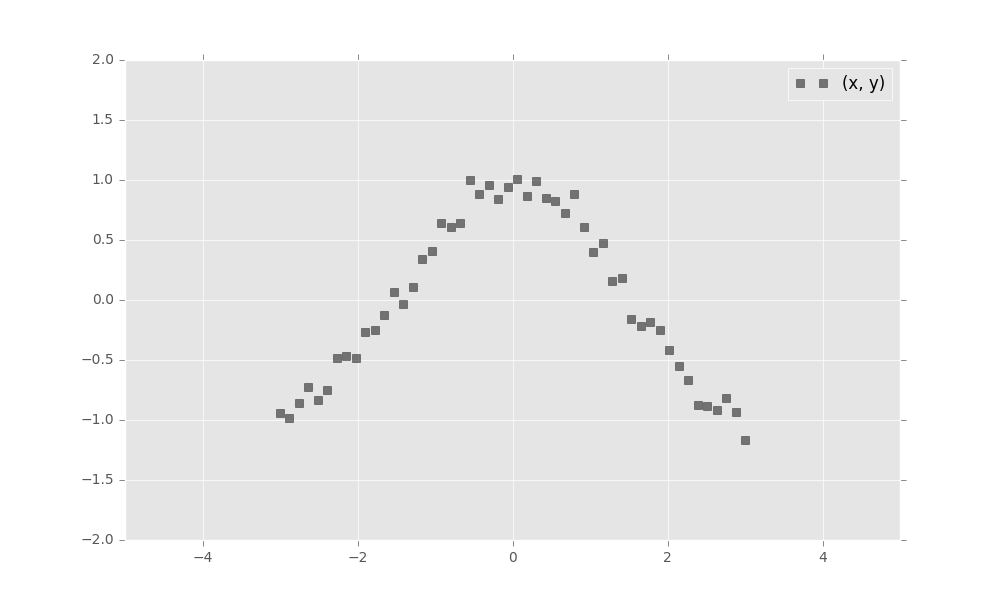
\includegraphics[width=700px]{images/getting-started-fig0.png}

Next, define a two-layer Bayesian neural network. Here, we
define the neural network manually with \texttt{tanh} nonlinearities.

\begin{lstlisting}[language=Python]
import tensorflow as tf
from edward.models import Normal

W_0 = Normal(mu=tf.zeros([1, 2]), sigma=tf.ones([1, 2]))
W_1 = Normal(mu=tf.zeros([2, 1]), sigma=tf.ones([2, 1]))
b_0 = Normal(mu=tf.zeros(2), sigma=tf.ones(2))
b_1 = Normal(mu=tf.zeros(1), sigma=tf.ones(1))

x = x_train
y = Normal(mu=tf.matmul(tf.tanh(tf.matmul(x, W_0) + b_0), W_1) + b_1,
           sigma=0.1)
\end{lstlisting}

Next, make inferences about the model from data. We will use variational
inference. Specify a normal approximation over the weights and biases.

\begin{lstlisting}[language=Python]
qW_0 = Normal(mu=tf.Variable(tf.zeros([1, 2])),
              sigma=tf.nn.softplus(tf.Variable(tf.zeros([1, 2]))))
qW_1 = Normal(mu=tf.Variable(tf.zeros([2, 1])),
              sigma=tf.nn.softplus(tf.Variable(tf.zeros([2, 1]))))
qb_0 = Normal(mu=tf.Variable(tf.zeros(2)),
              sigma=tf.nn.softplus(tf.Variable(tf.zeros(2))))
qb_1 = Normal(mu=tf.Variable(tf.zeros(1)),
              sigma=tf.nn.softplus(tf.Variable(tf.zeros(1))))
\end{lstlisting}

Defining \texttt{tf.Variable} allows the variational factors'
parameters to vary. They are all initialized at 0. The standard
deviation parameters are constrained to be greater than zero according
to a
\href{https://en.wikipedia.org/wiki/Rectifier_(neural_networks)}{softplus}
transformation.

Now, run variational inference with the
\href{https://en.wikipedia.org/wiki/Kullback–Leibler_divergence}{Kullback-Leibler divergence}
in order to infer the model's latent variables given data.
We specify \texttt{1000} iterations.

\begin{lstlisting}[language=Python]
import edward as ed

data = {y: y_train}
inference = ed.KLqp({W_0: qW_0, b_0: qb_0,
                     W_1: qW_1, b_1: qb_1}, data)
inference.run(n_iter=1000)
\end{lstlisting}

Finally, criticize the model fit. Bayesian neural networks define a distribution
over neural networks, so we can perform a graphical check. Draw neural networks
from the inferred model and visualize how well it fits the data.

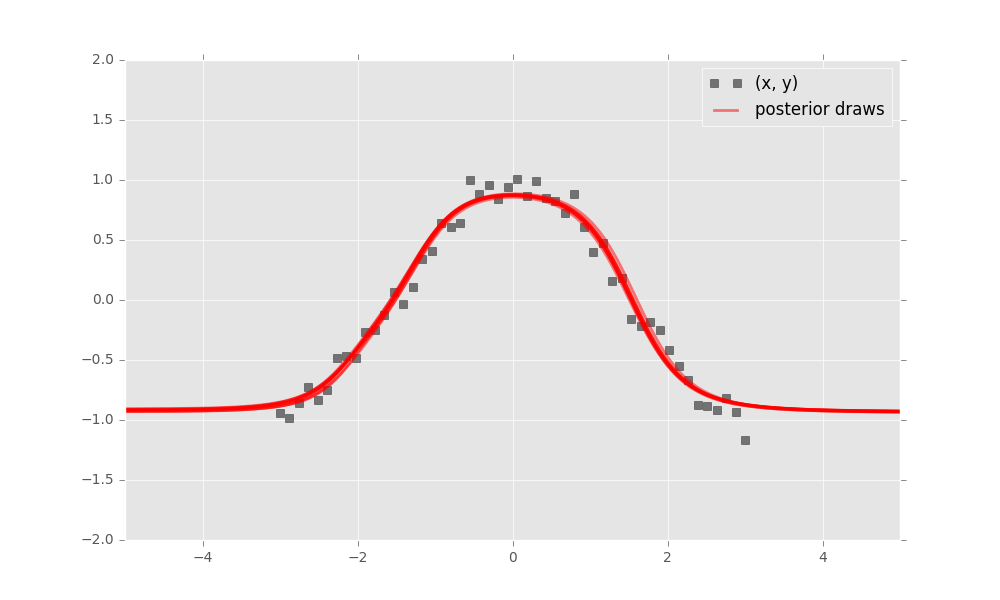
\includegraphics[width=700px]{images/getting-started-fig1.png}

The model has captured the cosine relationship between $x$ and $y$
in the observed domain.

To learn more about Edward, \href{/api}{delve in}!

If you prefer to learn via examples, then check out some
\href{/tutorials/}{tutorials}.
